\documentclass{article}
\usepackage{graphicx}
\begin{document}


\section{Introduction}


\label{sec:intro}
This document is used to describe the design of an architecture to make a robot learning the skill and be aware of the world, especially itself \textbf{autonomously}. It is more like a note to delight myself and sorting the thought of my own.

To be able to interactive with the external world, assuming that the robot can distinguish the signal of inputs e.g. camera image information and outputs e.g. sending the signal from its orign, the learning of sensorimotor map is critical. The developed mapping of sensorimotor makes the effect of action predictable or what action is needed when a desired effect comes into its mind. In robotics, we use the forward model to predict the effect of action and the inverse model to predict the action needed to a specified effect. The aim of the whole learning process is to work out an policy to perform the right action in right time, that is the responsibility of the predictor.

\section{Predictor}
\label{sec:predictor}

\subsection{Forward model}
\label{sec:forwardmodel}
The predicor will model and learn the world. Normally, there are two models to be learned, the forward model and the inverse model. Forward model mapping the next sensory state with the previous sensory and motor state. The forward model can be expressed by (\ref{eq:forwardmodel}).


\begin{equation}
  \label{eq:forwardmodel}
  S_{t+1} = F(S_t, M_t)
\end{equation}
$F$ is the function or the mapping of forward model.

For the learning of forward model, the online supervised learning algorithm would be used to optimize the parameters of $F$, therefore, the learning of forward model is equal to optimize $\hat{\theta}$, which is the parameters of $F$.
The examples of training forward model are the pairs of previous sensory and motor state and the next sensory input(state), $\{(S_{t-1}, M_{t-1}), S_t\}$. For instance, in a non-repeated one-dimension enviornment, the problem of mouse moving, where there is a mouse can move in three direction, e.g.left, right, and stay(-1,1,0), which is shown as Figure \ref{fig:mousemoving}. And the forward model should be able to predict the next state by the current state and the motion. 
\begin{figure}
  \centering
  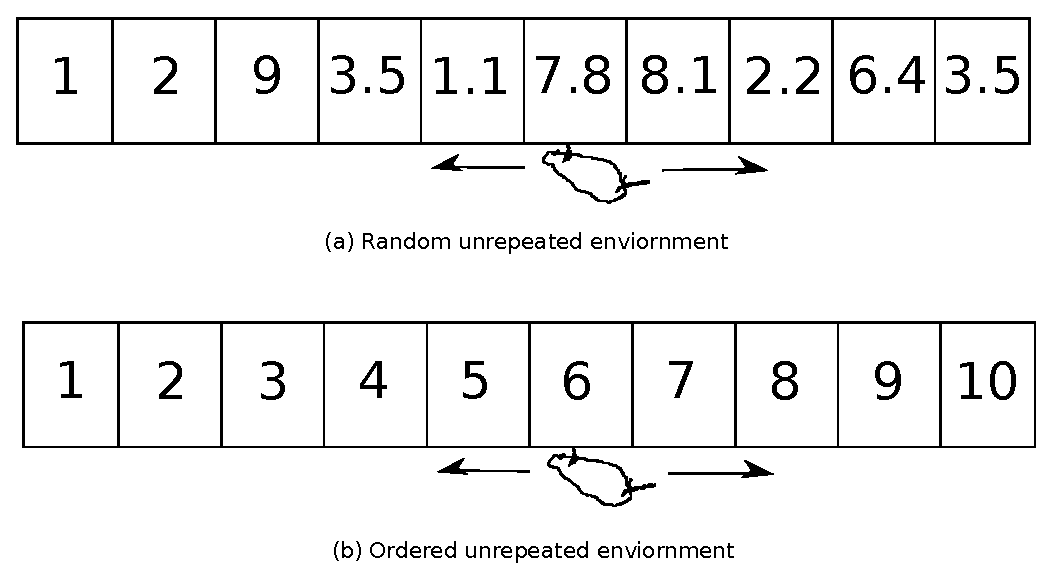
\includegraphics[scale=0.5]{fig/example_mouse.eps}
  \caption{Example of Mouse Moving}
  \label{fig:mousemoving}
\end{figure}
The model will fit a plane with a set of parameters, in this example, the plane of ordered environment is the exact plane, the one of random environment is a QUMIAN. The high-order parameters are needed, so the simple linear supervised learning can not approximate the plane well. 

The describtion of mechanical arm prediction HERE.....

The problem becomes more complicated when the dimension of sensory input and motor input become larger,e.g. the control of mechanical arm. In my project, the mechanical arm owns 7 DOF(Degree of freedom), that means, the dimension of motor input is 7 and it needs 7 joint angle sensors to sensor the status of the joints. The input size increses to be at least 15, including the bia. To apply the regular supervised learning algorithm, we have the architecture as Figure \ref{fig:archofnextarm}.
\begin{figure}
  \centering
  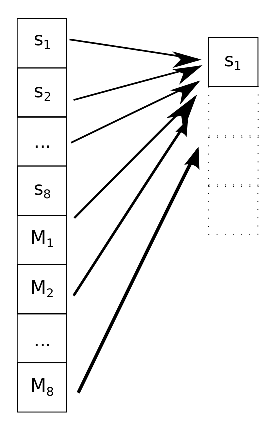
\includegraphics[scale=0.5]{fig/archofnextarm.eps}
  \caption{The architecture of predicting the next angle of the arm}
  \label{fig:archofnextarm}
\end{figure}

A new problem comes, which is, this architecture introduce too many extra inputs to predict the next states. Obviously, the next state $S_1(t+1)$ is only relative to $S_1(t)$ and $M_1(t)$, but this architecture use the other sensory and motor inputs to do the prediction. Although it is possible that the supervised learning algorithm will figure out the weights $\omega_{21}, \omega_{31},...,\omega_{n1}$ are all 0, it really increase the need of the quality and quantity of training examples. 

So it needs a mechanism to use the appropriate subset of the inputs to predict the subset of outputs. How to find the range of the subset? That is the main problem. The simplest method to solve it is to search within these subset of input and output, and to define the best matching pairs (e.g. Sensory 2 and motor 8 determine the next sensory state 3\&4).

\subsubsection{Granger Causality}
\label{sec:grangercausality}

This section is discussing the Granger causality.


\subsection{Inverse model}
\label{sec:inversemodel}


Inverse model will learn the mapping from the current state and the desired state to the action, that is, 
\begin{equation}
  \label{eq:reversemodel}
  M_t = I(S_t,S_d)
\end{equation}
$S_d$ is the desired state, $I$ is the inverse mapping.


\section{Actor}
\label{sec:actor}
If the robot choose the action randomly, that is, it applies a random policy, the input of training example is also very random. It is not an efficient way to train the model by the random data, as the number of example it needs can not be reached in life time, so an improved way is needed to optimize the acquisition of the examples. It is called the active learning, which is a way to acquire the data more intelligently and actively.

\subsection{Active learning}
\label{sec:activelearning}
The actor is an unit to implement the active learning algorithm. By using the actor, it choose the next action more directedly, that is to say, it is a better way to acquire much more high-quality data.
The mathmatical definition of the actor is a action selector, which is choosing the action as a specified sensory occurs,
\begin{equation}
  \label{eq:actormath}
  \pi_{\theta} : S \rightarrow A 
\end{equation}
where $\theta$ is the parameter set of policy $\pi$. Technically, the supervised learning algorithm can be used as a tool to evolve the actors. Importantly, the defintion of error of actor might be some possibilities, elborated as follows,
\begin{itemize}
\item The difference between the random action and the current actor. The better actor is, the large difference exists between the random action and current actor.
\item No idea yet

\end{itemize}

















\end{document}